\chapter{Solution perspectives}\label{chap:chap4}

\section{Envisioned approach}

The scheme represented by the Figure \ref{fig:envision}, resumes the envisioned approach.

\begin{figure}[h]
	\begin{center}
		\leavevmode
		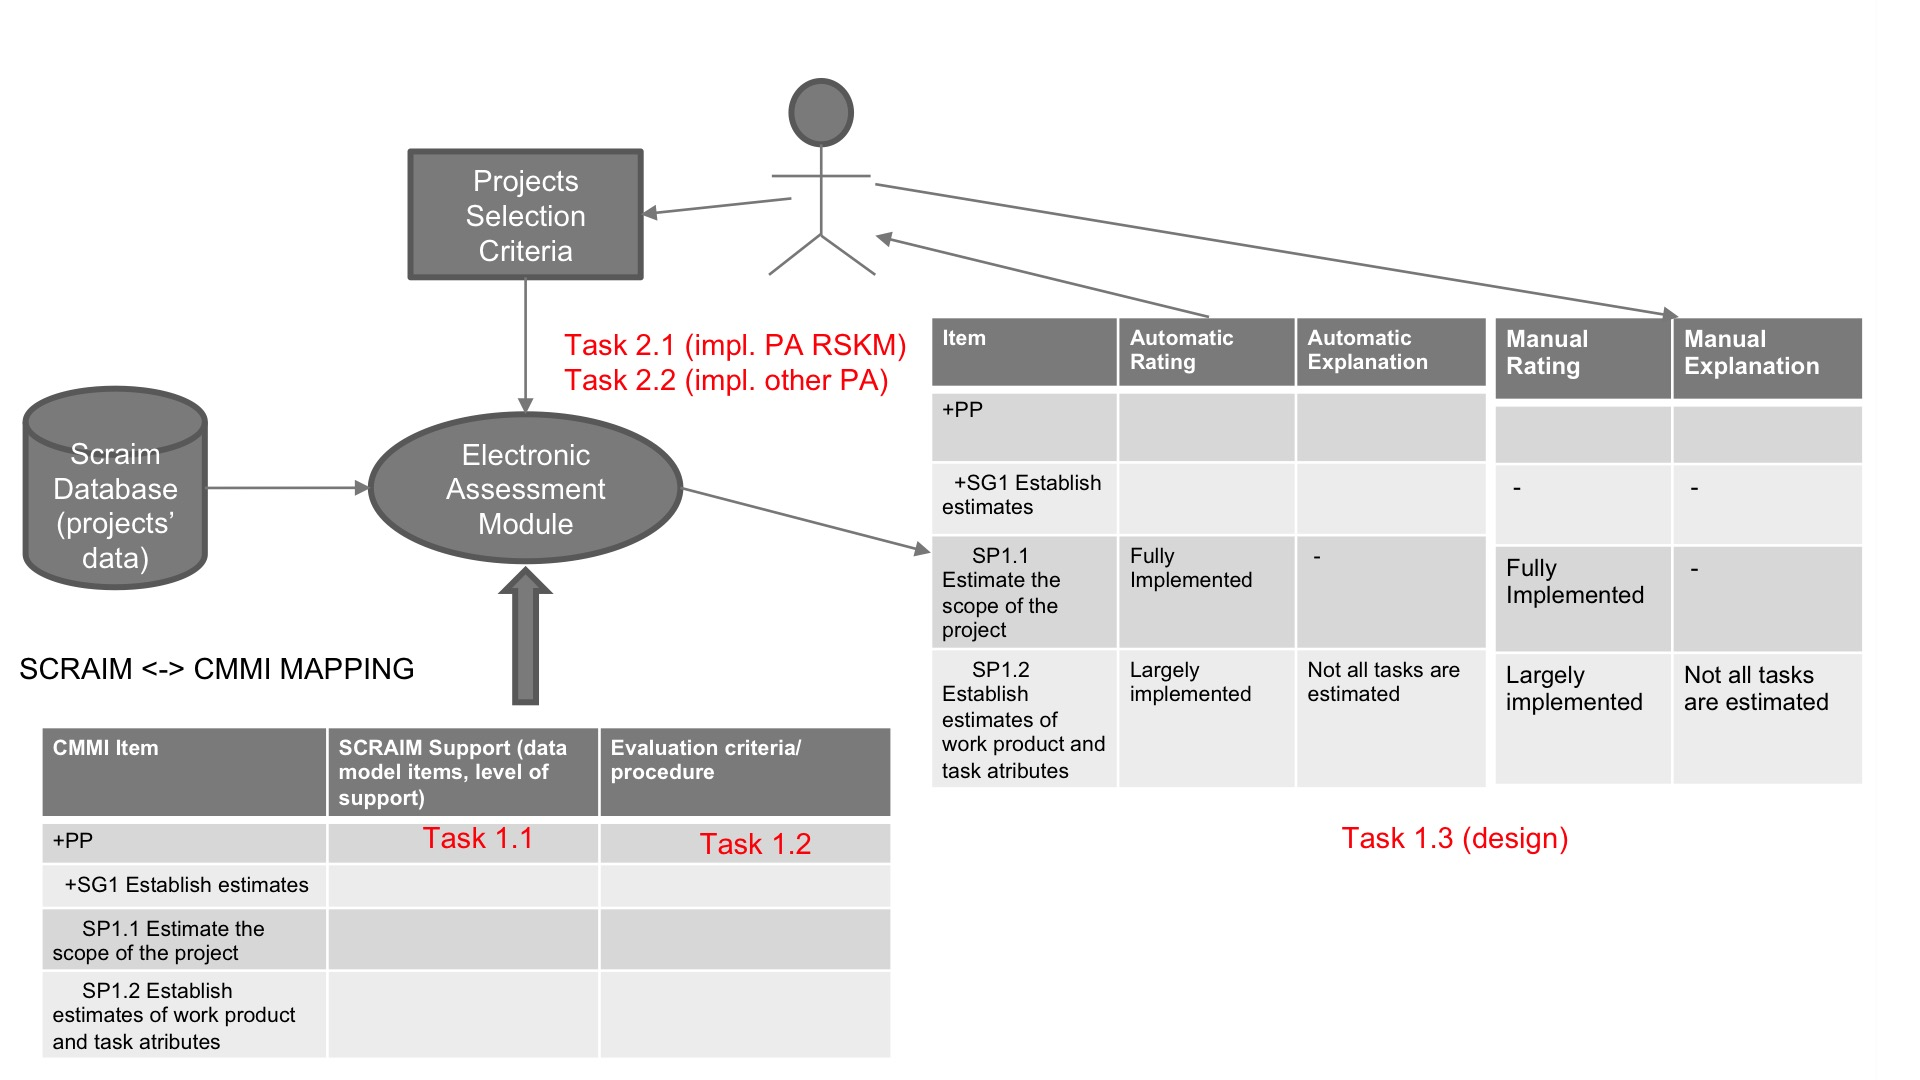
\includegraphics[width=1\textwidth]{envision}
		\caption{Envision approach scheme}
		\label{fig:envision}
	\end{center}
\end{figure}

The first step of this solution is make a CMMI-SCRAIM mapping where it is going to be evaluated the data model items and the level of support available on SCRAIM and match them to CMMI best practices.

Then will be made the design of the module, where will be evaluated on a top level the data from SCRAIM database taking for base the previous mapping.

In the last will be evaluated the results obtained by this automatic rating and compared to manual ratings taking for base real projects selected from SCRAIM.

\section{Work Plan}

The work plan consists in four main tasks that are:
\begin{itemize}
	\item Conception - that contains the CMMI-SCRAIM mapping, rule evaluation and analyze the results obtained.
	\item Implementation - consists in iterative SCRUM implementation.
	\item Validation - analyze the results obtained by the module produced comparing to real assessments.
	\item Thesis and article writing
\end{itemize}

The Gantt of is presented on the Figure \ref{fig:workplan}.

\begin{figure}[h]
	\begin{center}
		\leavevmode
		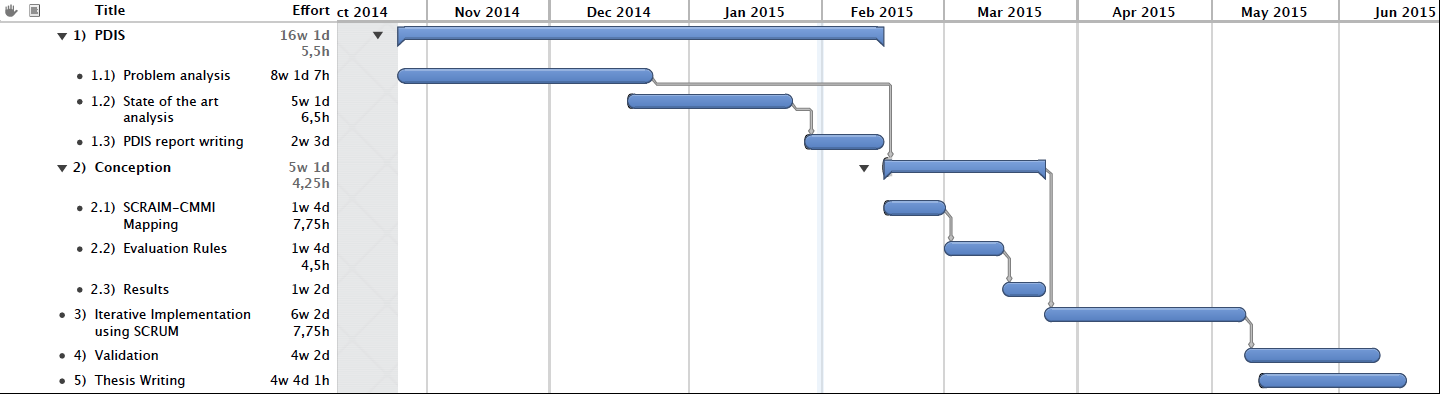
\includegraphics[width=1\textwidth]{workplan}
		\caption{Gantt Diagram}
		\label{fig:workplan}
	\end{center}
\end{figure}